\documentclass[10pt,twocolumn]{article}

%%% PACKAGE SETTINGS %%%
%% Font settings %%
\usepackage[T1]{fontenc}
\usepackage{charter}

%% Custom title page %%
\usepackage[center,small,sc]{titlesec}
\titleformat{\section}{\normalfont\fontsize{14}{14}\bfseries}{\thesection}{1em}{}
\titleformat{\subsection}{\normalfont\fontsize{12}{12}\bfseries}{\thesubsection}{1em}{}

%% Custom margins %%
\usepackage[nohead, nomarginpar, margin=.7in, foot=.35in]{geometry}
\setlength{\columnsep}{2em} % set space between two-column format
\setlength{\parskip}{.25em}

%% BibTeX citation pkg
\usepackage{cite}

%% Figures, listings with caption %%
\usepackage{hyperref}
\hypersetup{
  colorlinks,
  linkcolor={red!50!black},
  citecolor={blue!50!black},
  urlcolor={blue!80!black}
}
\usepackage{float}
\usepackage{graphicx}
\usepackage[font=normal,labelfont={bf,it},textfont={bf,it}]{caption}

\usepackage{lipsum}
\usepackage{xcolor}
\usepackage{textcomp}
\usepackage{listings}

\lstset{
  basicstyle=\small\ttfamily,
  aboveskip=1pt,
  belowskip=1pt,
  frame=single,
  captionpos=b,
  columns=flexible,
  keepspaces=true,
  linewidth=\columnwidth,
  breaklines=true,
  identifierstyle=\ttfamily,
  keywordstyle=\ttfamily\color[rgb]{0,0,1},
  commentstyle=\ttfamily\color[rgb]{0.133,0.545,0.133},
  stringstyle=\ttfamily\color[rgb]{0.627,0.126,0.941},
}

%%% DOCUMENT BEGINS %%%
\begin{document}
\begin{titlepage}
  \centering
  {\scshape\LARGE Vrije Universiteit Amsterdam\par}
  \vspace{1cm}
  {\scshape\Large Bachelor Thesis\par}
  \vspace{1.5cm}
  {\huge\bfseries <INSERT TITLE>\par}
  \vspace{2cm}
  {\Large\itshape Julien Couvy\par}
  \vfill
  supervised by\par
  Herbert Bos \& Cristiano Giuffrida
  \vfill
\end{titlepage}


\begin{abstract}

  \textbf{We present a proof of concept pseudo-compiler that translates a given
    exploit in any language to a return oriented programming payload for a
    target binary. In contrast to other works, we take advantage of the Turing
    completeness of the x86 mov instruction. By only having to handle mov
    instructions instead of the entire ISA, we reduce the complexity of crafting
  payloads while keeping, in theory, the same degree of expresiveness.}

  \textbf{We describe the fundamentals behind ROP attacks, and explain the
    functionning of our tool. In addition, we discuss its limitations and the
    results found using  sample test programs. Finally, we suggest ways to extend
  our work.}

\end{abstract}

\section{INTRODUCTION}
\lipsum[1-2]


\section{BACKGROUND}
\subsection{Code Injection}
Low level languages directly compiled to machine code such as C/C++ offer wider
possibilites of implementation without the cost of speed. However this freedom
has a price, programs written in these languages make use of powerful
instructions that can easily backfire on the user if used improperly. Such
programs are known to be vulnerable to numerous attacks diverting the control
flow during the execution of the program.

This paper will focus on one category of these attacks known as buffer
overflows. It is probably one of the most famous software vulnerability but
these attacks are still pretty common nowadays. A buffer overflow attack is an
anomaly where a program, while writing data to a buffer, overruns the buffer's
boundary and overwrites adjacent memory locations. In other words, a buffer
overflow condition exists when a program attempts to put more data in a buffer
than it can hold or when a program attempts to put data in a memory area past a
buffer.

Overflows can be used to modify return address or code pointers in order to
execute a malicious piece of code, sometimes already exisiting within the
program's space or injected by the attacker. They can be regrouped in two
types: stack-based overflows and heap-based overflows. Before going any further
it is required to understand how aprocess is organized in memory

\subsection{Process Memory Organization} 
First off we will briefly describe the
organization of processes in memory and recap what is the stack. Processes are
divided into three regions or segments: Text, Data and Stack.

\begin{figure}[h]
  \centering
  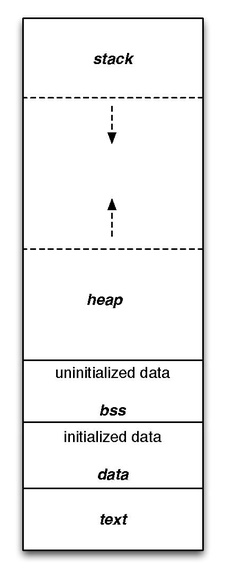
\includegraphics[scale=.85]{./graphics/stack_organization.jpg}
  \caption{Memory organization}
\end{figure}

The text segment also known as code segment is fixed by the program, it
includes the executable instructions - functions that make up the program (such
as main() if the program is written in C/C++) - and read-only data. This region
corresponds to the text section of the executable file. This region is normally
marked read-only and any attempt to write to it will result in a segmentation
violation.

The data segment is split in two parts: the initializated data part, simply
called data segment and the uninitialized data part also known asthe BSS
segment. The data segment contains the global variables and static variables
which have a pre-defined value and can be modified. The BSS segment contains
all global variables and static variables that are initialized to zero or do
not have explicit initialization in source code.

\medskip
\begin{lstlisting}[caption=Variable location in memory,language=C] 
// this static variable is stored in the BSS segment
static int bss_variable;
// this global variable is in the DATA segment
int data_variable = 42; 
\end{lstlisting}

Then we have the heap segment. It is the region where dynamic memory allocation
takes place. The heap area commonly begins at the end of the .bss and .data
segments and grows to larger addresses from there.

The final segment is called the stack. A stack is a contiguous block of memory
containing data. It is a LIFO (Last In First Out) data structure commonly used
in computer science. A register called the stack pointer (we will call it SP)
points to the top of the stack. In addition to the stack pointer, which points
to the top of the stack, a frame or local base pointer (FP or LP) is also
present which points to a fixed location within a frame. Its size is
dynamically adjusted by the kernel at run time. The CPU implements instructions
to PUSH onto and POP off of the stack. The stack consists of logical stack
frames that are pushed when calling a function and popped when returning. A
stack frame contains the parameters to a function, its local variables, and the
data necessary to recover the previous stack frame, including the value of the
instruction pointer at the time of the function call. Depending on its
implementation the stack will grow up or down. In the rest of this paper we
will consider that the stack grows downwards to reproduce the behavior of Intel
processors.

\subsection{Stack-based Overflows}
Back in November 1988, one of the first internet worm was born. Morris aka. the
Internet Worm was written and launched from the Massachussets Institute of
Technology by Robert Tappen, a graduate student at Cornell University. Despite
damaging the Internet for hundreds of thousands of dollars, it also permitted a
better understanding of a new variety of attacks called buffer overflows or
stack smashing attacks which until then had been mostly theoretical. They were
understood and partially publicly documented as early as 1972, however, Morris
was the first publicly documented exploit using this attack vector. The exploit
~\cite{one_stacksmashing_1996} relies on two factors:

Low level language's liberal approach to memory handling (mostly C back in that
time) Unix filesystem permissions (other OSes were also vulnerable) With
cautious manipulations, an attacker could grant himself unrestricted priviledge
to unpriviledged account or user. To explain the functionning of this attack we
will begin by an example of a typical stack behavior.

When invoking or exiting a standard C function, the procedure prolog or epilog
must be called, this involves saving the previous variables and allocating
space for the new variables; and vice-versa when the function exits. The
previous FP is pushed, a new FP is created and SP operates with respect to its
new local variables.

Using the below code as an example depicts a straightforward
situation:

\subsection{Return Oriented Programming}
In this section we will introduce the concept of Return Oriented Programming
(ROP)~\cite{roemer_return-oriented_2012}. Traditionnally code injection attacks
relies on diverting the normal control flow of a program and introduce
arbitrary, usually malicious, behavior. The principal attack vector for
injections is a stack buffer overflow, though many other alternatives were
invented such as buffer overflows on the heap, integer overflows... To achieve
his goal, the attacker must (1) subvert the program's control flow from its
normal course, and (2) redirect the program's execution. In traditional
stack-smashing attacks, an attacker completes the first task by overwriting a
return address on the stack, so that it points to code of his choosing, the
\textit{shellcode}, rather than to the function that made the call. However,
this kind of attacks was discovered a long time ago and multiple defenses were
set up against them: (W+X, DEP...)

Return oriented programming shares the same ideas than return-to-libraries
attacks. An attacker who managed to redirect the program's control flow can
force it to execute a payload without introducing any new code; there are no
code injections at all. Instead, the attacker re-uses code already present in
the binary whether in libraries (for return-to-libc attacks for example) or in
executable memory. The latter is where ROP differs from return-to-libraries
attacks. To some extend ROP can be seen as a generalization/refinement of
return-to-libraries attacks.

Return oriented programming is a relatively new technique that evades most code
injection defenses such as W$\oplus$X. Most recent malwares use ROP to bypass
those defenses and deliver their payload. It is important to note that ROP is
not flawless, the scientific community has already found counter measures and
is still working on preventing such attacks. (++ SEARCH FOR RELATED PAPERS).
The technique consists of aggregating malicious computation by linking together
short code snippets called \textit{gadgets} already present in the program's
address space (similary to how return-to-libc attacks uses pre-written
functions in libc).  A \textit{gadget} ends in a ret instruction and is located
in a subroutine within the exisiting program and/or shared library code.
Chained together, these gadgets allows an attacker who controls the call stack
to build and execute his payload. Because the executed code is stored in memory
marked executable, the W$\oplus$X defense will not prevent it from running. The
following figure shows the call stack state with a ROP attack (taken from
here~\cite{bletsch_jump-oriented_2011}).

While this technique appear simple in theory, it is much more complex in
practical use. First, finding proper gadgets in the program's address space is
no simple task. Once an attacker has found suitable instructions, he has to
find a way to properly link them altogether in order to create his payload. All
this work was done manually for a time and it is safe to say that it was a
lenghty labour. To solve this issue, we saw the appearance of the first return
oriented programming compilers such as Q, ROPC, Mona and others... However,
none of them are still completely reliable. Actually, most of them are only
proof of concepts and do not work in a real-life situations: one will give up
on Turing completeness, another would not provide any verification procedure
(essential as some gadgets can be semantically incorrect)...

What we are trying to achieve is : ........
\section{RELATED WORK}
\lipsum[1]

\section{MOV2ROP}
\lipsum[1]
\subsection{Gadget Extraction}
\lipsum[1]
\subsection{Payload Treatment}
\lipsum[1]
\subsection{Instruction Analysis}
\lipsum[1]
\subsection{Gadget chaining}
\lipsum[1]
\subsection{Limitations}
\lipsum[1]

  
\section{RESULTS \& CONCLUSION}
  We tested our tool on two sample programs written in C. For each case, the
  target binary is the program compiled with a static version of \textit{glibc}.

  We demonstrated a simple yet powerful way to craft return oriented payloads
  which are still to this day a strong attack vector. By exploiting the Turing
  completeness of mov instructions coupled with a mov-compiler, we greatly
  simplified the work needed to implement the exploits. The potential of ROP
  attacks is mainly hindered by the complexity of crafting gadget chains in real
  life scenarios. However, it is possible to find automated ways to handle this
  work making ROP attacks an even bigger threat.

\section{FURTHER WORK}
\lipsum[1]

\section{REFERENCES}
\begingroup
\renewcommand{\section}[2]{}
\bibliographystyle{acm}
\bibliography{references}
\endgroup

\appendix
\clearpage
\section*{Appendix}
\begin{table}[!ht]
  \centering
  \lstinputlisting[caption=Fibonacci.c,language=C]{../test_programs/fibonacci.c}
  \medskip

  \begin{tabular}{l|l|l}
    \textbf{Total Instructions} & \textbf{1270} & \textbf{100\%} \\ \hline
    Supported                   & 1042          & 82\%           \\ \hline
    Supported (w/o offsets)     & 962           & 75\%           \\ \hline
    Not supported               & 228           & 17\%          
  \end{tabular}%
  \label{result-fibo}
  \caption{Statistics on fibonacci.c}

  \bigskip

  \lstinputlisting[caption=Hanoi\_towers.c,language=C]{../test_programs/hanoi_towers.c}
  \medskip

  \begin{tabular}{l|l|l}
    \textbf{Total Instructions} & \textbf{2054} & \textbf{100\%} \\ \hline
    Supported                   & 1071          & 82\%           \\ \hline
    Supported (w/o offsets)     & 1579          & 76\%           \\ \hline
    Not supported               & 353           & 17\%          
  \end{tabular}%
  \label{result-hanoi}
  \caption{Statistics on hanoi\_towers.c}
\end{table}

\end{document}
